\documentclass{beamer}
\usepackage{beamerthemesplit}
\usetheme{Boadilla}
%%\usecolortheme{default}
%% \definecolor{meerkat-blue}{HTML}{0090CA}

%% \setbeamercolor*{titlelike}{bg=meerkat-blue,fg=black}
%%  \setbeamercolor*{title page}{bg=meerkat-blue,fg=black}
%%  \setbeamercolor*{block title}{bg=meerkat-blue}
%%  \setbeamercolor*{palette secondary}{use=structure,fg=white,bg=meerkat-blue}
%%  \setbeamercolor*{palette tertiary}{use=structure,fg=white,bg=meerkat-blue}
%%  \setbeamercolor*{palette quaternary}{use=structure,fg=white,bg=meerkat-blue}

 \setbeamertemplate{navigation symbols}{}%remove navigation symbols
\title[Public Health Surveillance]{Technical introduction to Public Health Surveillance System}
\author{Gunnar and Jonathan (Jyri, Mikolaj, Tomek, Ziad)}
\institute[WHO]{World Health Organisation}
\date{\today}



\begin{document}

\begin{frame}
\titlepage
\end{frame}

\begin{frame}
\tableofcontents
\end{frame}

\section{Overview and Introduction}
%% 20 min

\begin{frame}
  \frametitle{Mission statement}

  \begin{block}{Public health surveillance mission statement}
    To enable real-time case-based surveillance at the health facility level that improves public health and clinical decision making at all levels of the health system.
  \end{block}
  \vspace{10pt}
  To this end the we want to develop secure and reliable technical solutions that fulfill the following principles:

  
  \begin{itemize}
  \item Configurable services
  \item A micro-service architecture
  \item Supporting multiple data source and multiple data outputs
  \item Open source
  \end{itemize}
\end{frame}  

\begin{frame}
  \frametitle{Short history}
  \begin{itemize}
  \item Spring 2014: Pilot project with 50 clinics Communicable Diseases
  \item April -- September 2015: National scale up to over 300 clinics
  \item Spring 2016 RMS system started
  \item NCD Scale up June 2016
  \item Mental health March 2017
  \end{itemize}
\end{frame}

\section{Principles of implementation}

\begin{frame}
  \frametitle{Microservices Architecture}
  We aim to design the system so that we have a system of loosely coupled smaller services performing a self contained range of functions.

  \begin{itemize}
  \item Each component has a clearly defined limited scope
  \item Each component should be independently deployable
  \item Components are mainly coupled through APIs
  \item Made much easier by Docker
  \end{itemize}

  Benefits:

  \begin{itemize}
  \item Each component can be developed independently
  \item Can make different design decisions for each component
  \item Components can be easily replaced if needed
  \item Separation of responsibilities and non repetition of code
    \end{itemize}
\end{frame}

\begin{frame}
  \frametitle{Open Source}
  We only use open source components and release all code as open source.

  \vspace{30pt}
  
  Using open source brings many benefits:

  \begin{itemize}
  \item No licensing costs etc. 
  \item Other groups can use and improve our software
  \item Can determine in detail how everything works if needed
  \item Much industry leading software is open source
  \end{itemize}

\end{frame}
\begin{frame}
  \frametitle{Continuous Integration}
  We develop our software on a continuous release cycle that can always be deployed.\\
  \vspace{5pt}
  Made possible by:
  \begin{itemize}
  \item Version control via git
  \item Unit-testing and automatic testing on code push (Travis)
  \item Nightly builds of development branch
  \item Automatic build and deploy process
  \item Flexible infrastructure in the cloud
  \end{itemize}
  \vspace{5pt}
  Benefits:
  \begin{itemize}
  \item Faster deployment of needed changes
  \item Continuous feedback on changes and incremental improvements
  \end{itemize}

\end{frame}




\section{Technical Structure}
%% 30 min
\begin{frame}
  \frametitle{Current Data Flow}
  \begin{center}
    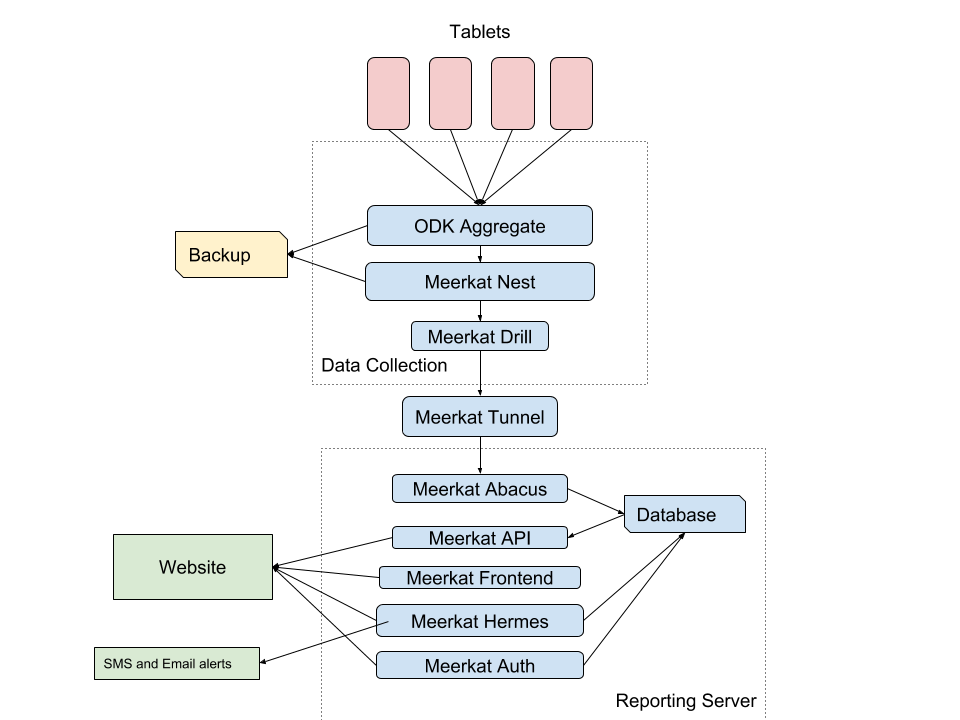
\includegraphics[width=9cm]{data_flow.png}
  \end{center}
\end{frame}


\begin{frame}
  \frametitle{Data Flow}
  The main function of the software is to get the information from the tablets to the users in a useful format. \\
  \vspace{10pt}

  We want to support many different sources of data and different formats. \\

    \vspace{10pt}
  
  E.g: Gender might be coded as M/F in variable gen in one form and as male/female in variable pt1./gender in another. \\

    \vspace{10pt}
  
    To overcome this we process all the raw data using configurable codes so that both way of specifying gender can be combined. The end point of this is a clean data table which can easily be used for aggregation. \\

    \vspace{10pt}
    This data can then be used to power the websites and other data displays

    
  \end{frame}


\subsection{Data Collection}

\begin{frame}
  \frametitle{Data Collection}
  Data collection modalities:
  \begin{itemize}
  \item Forms submitted from tablets (Main modality)
  \item Automatic status messages from tablets (Under development)
  \item Uploading spreadsheets (Experimental feature)
  \item Data from other sources via APIs (Future)
  \end{itemize}

  \vspace{10pt}
  All collected data will be stored on the servers in MoH/RMS and is owned by them. 
\end{frame}


\begin{frame}
  \frametitle{Data collection from tablets}
  \begin{itemize}
  \item Android tablets that run custom version of ODK Collect
  \item Automatic synchronization of app and forms
  \item Automated configuration
  \item Forms are created in Excel (XLS forms)
  \item http://xlsform.org/
  \item Automatic status messages via Google Cloud Messaging
  \item Tablet management needs to be improved
  \end{itemize}
\end{frame}
\begin{frame}
  \frametitle{Data Collection Server}
  \begin{itemize}
  \item Server in MOH an RMS Data Centres
  \item Ubuntu Linux operating system
  \item Full disk encryption and modern security
  \item Recently updated to enable real-time data. Now using docker.
  \item Runs ODK Aggregate software
  \item Java application running in Tomcat behind Nginx
  \item Daily backup or real time backup
  \item Meerkat Nest anonymises the data and sends it to a message queue (for real time)  
  \end{itemize}
\end{frame}

\subsection{Data processing}
\begin{frame}
  \frametitle{Data Processing}
  This service starts with the raw anonymised data and provides aggregated data for display
  \begin{itemize}
  \item Configurable codes are used to translate raw data into useful data
  \item These codes provide a flexible way of giving meaning to the data.
  \item Support: Matching, calculated values, number in interval, multiple conditions etc
  \item Data processing tools also deal with important meta data like locations and tablets.
  \item Data is localised by matching on device-ids or by gps
  \item Provide an API that gives access to data
  \item Supports a wide range of aggregated data views.
  \item Data processing has two components Abacus and API
  \end{itemize}
\end{frame}



\begin{frame}
  \frametitle{Meerkat Abacus}
  \begin{itemize}
  \item Python package that imports raw data and meta data and processes the data to the finished data table
  \item Reads data from message queue for real time (currently ~10 m) soon ~ 1m. 
  \item Uses a PostgreSQL database for support of JSON 
  \item When processing data alerts are identified and sent out
  \item Supports both single and threshold alerts
  \item Supports codes based on linking multiple form entries
  \item Data sources, locations, codes and links configurable
  \item https://github.com/meerkat-code/meerkat\_abacus
  \end{itemize}

\end{frame}

\begin{frame}
   \frametitle{Example}
  \begin{center}
    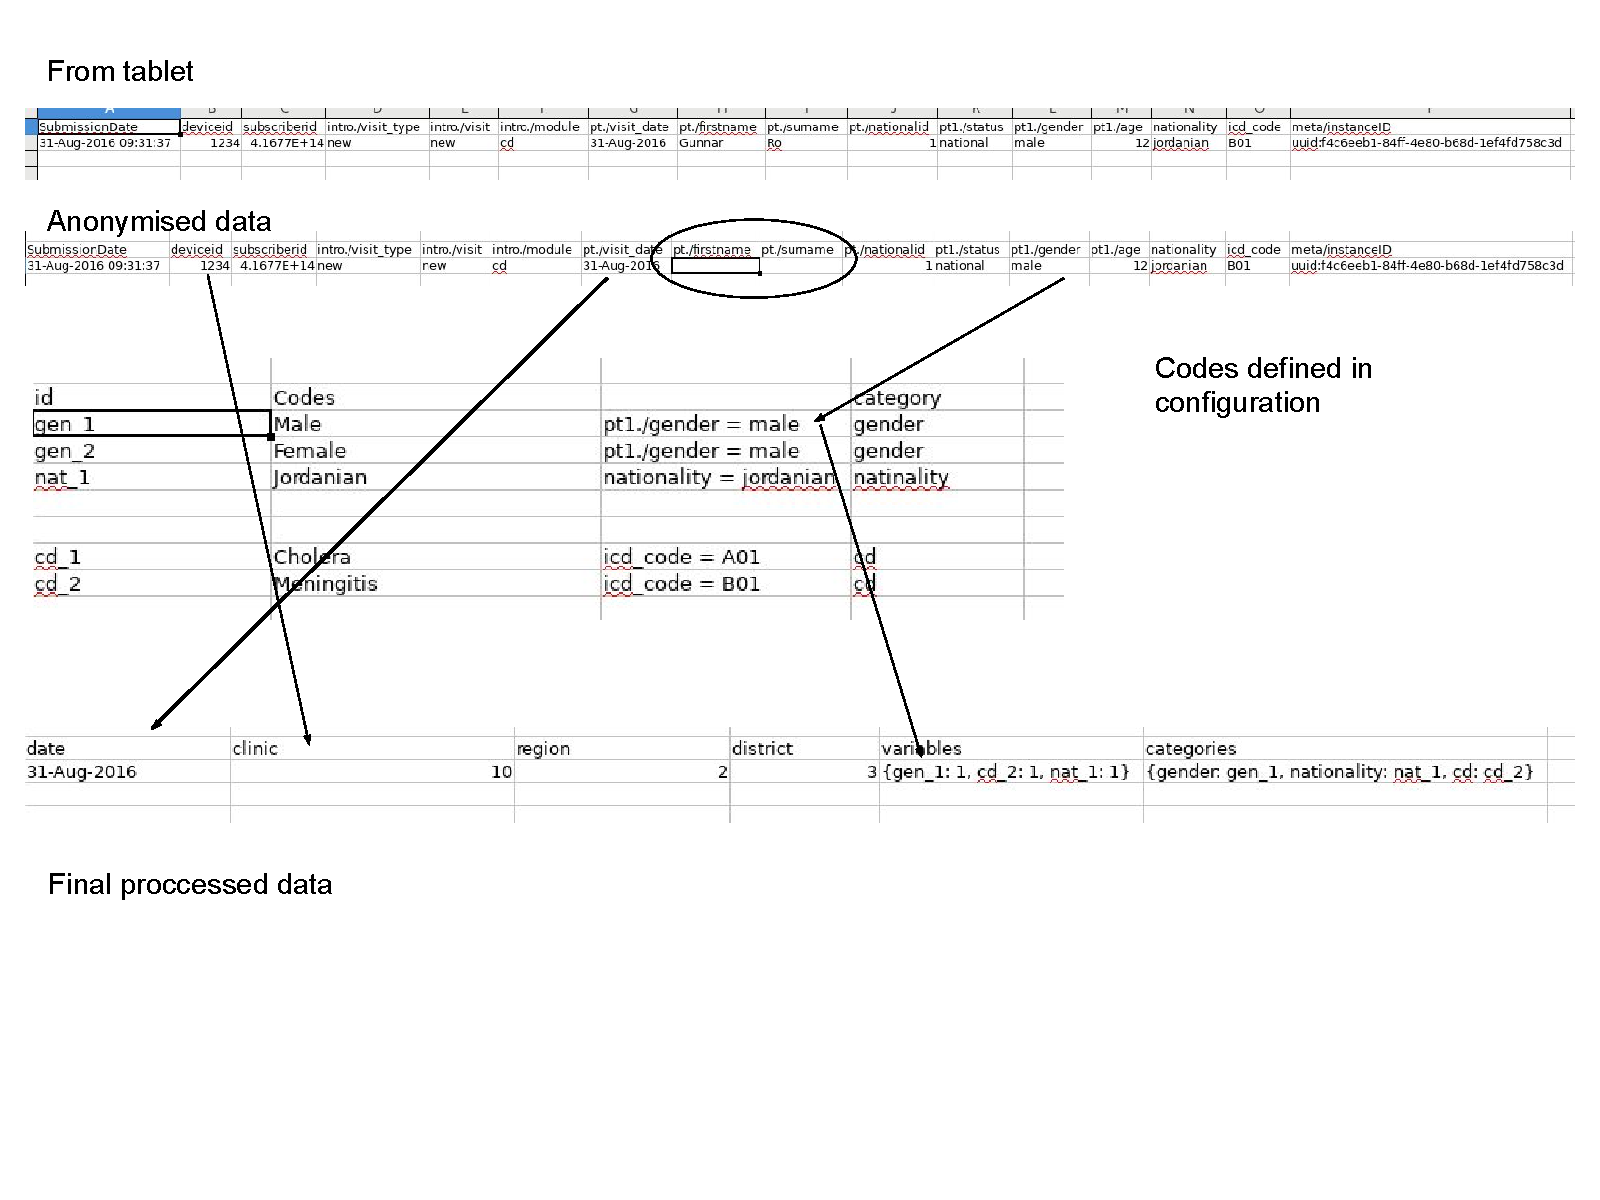
\includegraphics[width=11cm]{ex.pdf}
  \end{center}

\end{frame}

\begin{frame}
  \frametitle{Databases in the Meerkat System}

  Many databases are used in the Meerkat system. We use PostgreSQL for all.
  \begin{itemize}
  \item ODK Aggregate database - Database for ODK aggregate, follows ODK schema. Raw data
  \item Nest database - {\bf Truth database} - raw data and anonymised data
  \item Persistent database on reporting server
  \item Main meerkat database - Processed data - ``recalculated'' on each startup
  \item Notifications and authentication databases
  \end{itemize}
  Current structure designed for cloud solution. Re-engineering needed?
\end{frame}

\begin{frame}
    \frametitle{Meerkat Api}
    \begin{itemize}
    \item Python package that provides an HTTP rest API to query data
    \item Based on Flask
    \item Used Pandas for some of the data aggregations
    \item Supports aggregation over time and location
    \item Mapping of cases, incidence rates and clinics
    \item Supports many reports
    \item Supports explore data functionality
    \item Supports downloading the raw data using a Celery as task runner
    \item For the API only the processed data is used
    \item https://github.com/meerkat-code/meerkat\_api
    \end{itemize}
\end{frame}

\subsection{Web interface}
\begin{frame}
  \frametitle{Meerkat Frontend}
  \begin{itemize}
  \item The website you can see at iers.moh.gov.jo
  \item Written in Python and HTML, JS, CSS
  \item Uses many open source libraries. E.g bootstrap and Highcharts
  \item Includes public homepage and then a private technical page
  \item Technical page includes data on demographics, morbidity, completeness, PIP and alerts
  \item Very configurable, can change the number and content of the tabs
  \item The technical site also includes download data, explore data and reports
  \item https://github.com/meerkat-code/meerkat\_frontend
  \item {\bf Meerkat Hermes}: Separate microservice to sends email and SMS notifications and administer notifications
  \end{itemize}
\end{frame}
\begin{frame}
  \frametitle{Authentication}
  \begin{itemize}
  \item The frontend supports many different user accounts and access levels
  \item Each component and each tab can have different access levels. 
  \item Authentication is implemented as a separate microservice
  \item Written in Python and HTML, JS, CSS
  \item Uses encrypted JSON webtokens to communicate access rules
  \item We have user accounts and roles
  \item Completely flexible access role network
  \item https://github.com/meerkat-code/meerkat\_authentication
  \end{itemize}
\end{frame}


\begin{frame}
  \frametitle{Example}
  {\Huge Example on whiteboard}
\end{frame}

\begin{frame}
  \frametitle{Documentation}

  All Meerkat components are documented to various degrees. The documentation will be in the handover and can be access at : http://meerkat-docs.s3-website-eu-west-1.amazonaws.com/
  
\end{frame}

\begin{frame}
  \frametitle{Software review}
  \begin{itemize}
  \item Operating system: Linux (mainly ubuntu)
  \item Containerisation: Docker
  \item Python, Flask, Celery, SqlAlchemy
  \item JS (gulp, highcharts, bootstrap, jquery), HTML, CSS
  \item Message queues: RabbitMQ
  \item Databases: PostgreSQL, Redis
  \item Version control: git 
  \end{itemize}
\end{frame}
\begin{frame}
  \frametitle{Important programming libraries}
  {\bf Python:} \\
  Flask : micro-framework for web programming \\
  SqlAlchemy: Database abstraction \\
  pandas: Data analysis \\
  shapely: GIS \\

  \vspace{10pt}

  {\bf Javascript:} \\
  jQuery: DOM manipulation \\
  bower: asset management \\
  gulp: task runner \\
  
\end{frame}

\subsection{Infrastructure}
\begin{frame}
  \frametitle{Meerkat Infrastructure}
  \begin{itemize}
  \item Use docker for containerisation for both production and development
  \item A github repository for every country and a demo country
  \item Data collection server is physical server in MoH and RMS
  \item Website moving to local server in MOH this week
  \item We use Travis for automatic testing
  \end{itemize}
\end{frame}

\begin{frame}
  \frametitle{Technical Debt from moving to local server}
  \begin{itemize}
    \item Many new features that have not been tested very well. Will lead to {\bf instability}
    \item Development website. It is very useful to have a development version of the online framework where any changes can be tested before being deployed
    \item Improve and customise utilities and tools. 
    \item Downtime for deployment. Any deployment will take  ~3 hours. The site will not be working proplery during this. 
    \item There is no redundancy for high availability. If there are any hardware failures for any of the servers there are no replacements ready to be used. 
    \item The infrastructure is now more ad-hoc and requires manual setup.
  \end{itemize}
\end{frame}

\begin{frame}
  \frametitle{Training}

  {\bf What do you want to cover?}

  \begin{itemize}
  \item {\bf Linux and Docker}
  \item {\bf Creating forms}
  \item {\bf PostgreSQL Database}
  \item Python Programming
  \item Git
  \item Web programming
  \item Data analysis
  \item Meerkat Storage Solutions
  \item Linux networking and security
    \item Meerkat System Excersises

  \end{itemize}
\end{frame}
\begin{frame}
  \frametitle{Introductions and program}


  {\large Today:}
  \vspace{5pt}
  
  Introduction and system architecture
  
  {\bf Discussion} about training goals
  
  Forms
  
  {\it Lunch}
  
  Linux Training
  
  \vspace{30pt}  
  {\large Tomorrow:}
         
  \vspace{5pt}  
  Debugging running Meerkat System
  
\end{frame}  
  


\end{document} 
